\section{Materials and Methods}\label{sec:methods}\label{sec:methodology}

This section presents the methodology adopted in this study. Figure~\ref{fig:workflow} provides an overview of the methodological flow adopted in this study. The diagram highlights each step of the process, illustrating the flow from data acquisition to model optimization and evaluation.

\begin{figure}[ht]
    \centering
    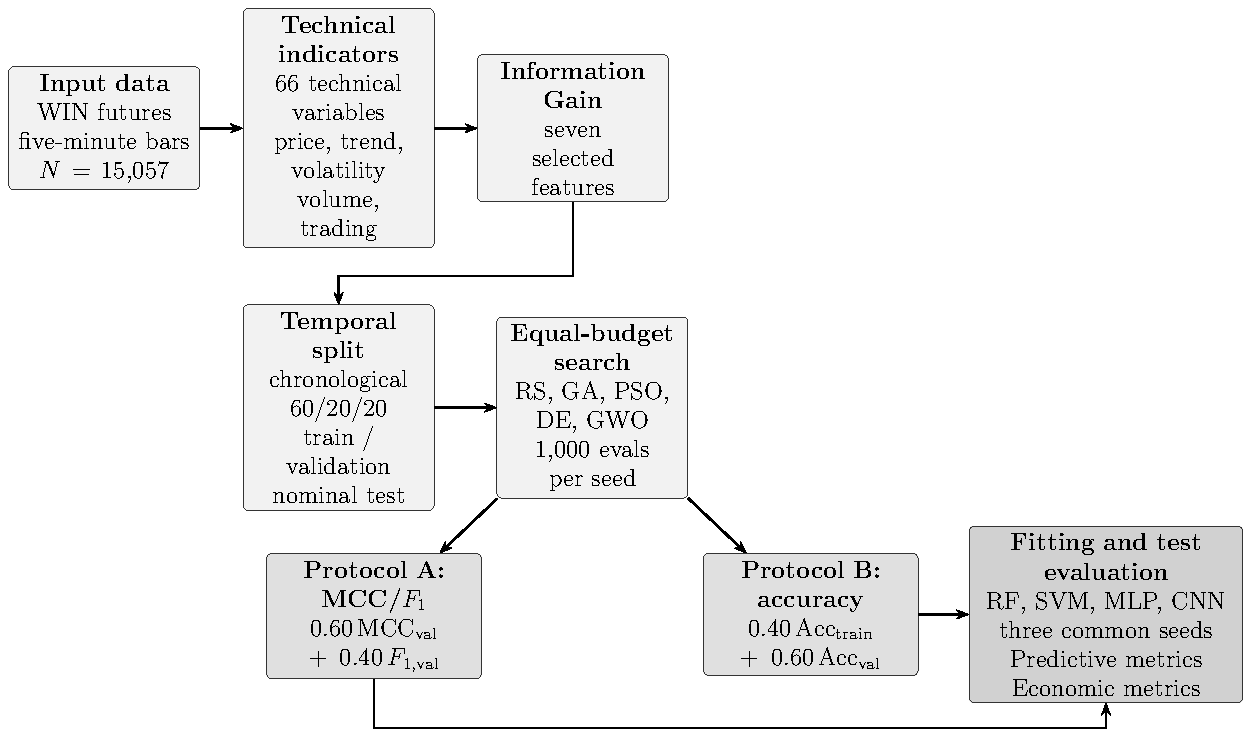
\includegraphics[width=0.90\linewidth]{figures/methodology_workflow_vector.pdf}
    \caption{Overview of the proposed methodology. The benchmark reuses the precursor’s fixed
Information-Gain representation while enforcing a chronological split, equal optimizer budget, and
two separated validation objectives.}
    \label{fig:workflow}
\end{figure}

\subsection{Input Data}
\label{sec:data}

The data used in this study were obtained from BovDbV2 \cite{souza2024dataset}, an extension of the original BovDb \cite{cardoso2022bovdb}. The database provides publicly available and pre-processed B3 market data for research purposes, covering listed assets from 1995 to 2024. BovDbV2 additionally includes intraday observations aggregated into 5-minute intervals for the first half of 2024, enabling the analysis of short-horizon market behaviour.

For the present study, the analysis focuses on Mini Ibovespa Futures (WIN) contracts traded between January and June 2024. The selected contracts correspond to the most actively traded maturities over the analyzed period: WING24 and WINJ24 in January--February, WINJ24 and WINM24 in March--April, and WINM24 and WINQ24 in May--June. After preprocessing and construction of the modelling dataset, the final sample contains 15,057 chronological observations.

The explanatory variables are technical indicators computed from completed five-minute price and volume bars. The binary regime labels (0, downtrend; 1, uptrend) are generated from peak-and-trough structure detected on hourly candles resampled from the five-minute price series. The detector groups consecutive bullish and bearish hourly candles, locates the highest or lowest close within each run, refines that pivot to the corresponding extreme five-minute close, and checks the following hourly interval for a more extreme close. The resulting pivot states are assigned to five-minute observations and carried forward; the initial segment is assigned retrospectively from the first detected pivot. We reproduced this procedure against the archived label database and obtained exact agreement for all 23,181 stored rows. In the modeling dataset, each five-minute feature row is paired with the next retained regime-label row for the same ticker, $y_{i,t} = r_{i,t+1}$. This alignment agrees with the archived label database for all 15,053 rows with a successor, including 196 session-final rows whose successor is in the following session. Four final rows, one per ticker series, have no successor and retain their contemporaneous label. Thus, the benchmark is a next-observation regime-prediction task, with four terminal-row exceptions. Predictions are available after bar $t$ closes; the economically aligned entry is at the open of bar $t+1$. The hourly pivots and their confirmation are retrospective, so this one-bar shift does not make the target itself causal.

All observations are kept in their original chronological order. The first 9,034 observations are assigned to the training set, the following 3,011 observations to the validation set, and the final 3,012 observations to the nominal test set. No random shuffling is performed. Because the target is shifted by one retained row, however, one training observation at the split boundary is paired with a validation-period label, and two validation observations are paired with test-period labels. These three boundary observations were retained in the reported experiments; thus, the test block is chronologically subsequent, but its labels are not fully isolated from model selection. A cutoff audit that reran the recovered label routine using only price history available through each cutoff found no label changes among the other 9,032 training and 3,008 validation targets checked. This audit addresses retrospective changes to the recovered pivot labels, not the three direct one-row crossings or the longer confirmation horizon of the pivot rule. In addition, four final per-ticker rows have no next retained observation and use their contemporaneous source label. Results should therefore be interpreted with these boundary and terminal-row exceptions in mind.

\subsection{Generation of Technical Analysis Indicators}
\label{sec:indicators}

Technical indicators were built from the intraday dataset to capture short-term price changes. Key metrics—Simple Moving Average (SMA), Exponential Moving Average (EMA), and Standard Deviation—were calculated using short time windows (3, 5, 7, and 9 periods) to enhance sensitivity to rapid market shifts, where significant moves can happen in minutes \cite{hunter1986exponentially}.

To capture changes in trend slope and momentum, attributes derived from the differences between calculated moving averages were also constructed. For example, the difference between the 7-period SMA and the 3-period SMA is defined in Eq. (1) as:

\begin{equation}
\text{SMA}_{7-3} = \text{SMA}_{7} - \text{SMA}_{3},
\end{equation}

A central preprocessing step consisted of normalizing the technical indicators \cite{singh2022feature}, as well as the opening and closing prices, in order to place all variables on a common numerical scale. For each 5-minute intraday window, a min–max–type scaling was applied, in which each feature was transformed according to Eq. (2):

\begin{equation}
\text{Feature}_{\text{norm}} = \frac{\text{Feature} - \text{Low}}{\text{High} - \text{Low}}.
\end{equation}

Where \textit{High} and \textit{Low} correspond to the maximum and minimum prices observed within the same 5-minute interval, and \textit{Feature} denotes any technical indicator or price-based variable being normalized. This transformation maps the features predominantly to the interval $[0,1]$, while preserving their relative positions within the intraday price range, thereby reducing the impact of heterogeneous attribute scales and facilitating the learning of machine learning models. This normalization procedure, combined with historical information on open, high, low, average, close, bid, ask, trade volume, and number of shares, results in a total of 66 constructed features.

\subsection{Feature Selection Method}
\label{sec:featureselection}
The predictive pipeline incorporates a structured feature selection stage based on technical analysis indicators. Following the approach proposed in \cite{souza2024dataset}, multiple selection strategies are evaluated to identify the most informative feature subsets, thereby enhancing model discrimination while reducing redundancy and noise inherent in high-dimensional financial data.

In the precursor, feature-selection strategies included filters and wrappers. The Information Gain ranking was produced in WEKA using only the chronological training partition (January--March 2024), separated by the number of five-minute observations in that interval; the April--June test partition was excluded, as confirmed by the researcher. The ranking was then recorded as a fixed list in the Python workflow. Its first seven features form the compact representation used here. The present benchmark applies that inherited mask without re-estimating selection on its own training partition, so its conclusions remain conditional on the selected representation. The original WEKA project/output is not archived, but the selected feature list and the subsequent train/test data split are preserved in the project files.

The selected features, ranked by their Information Gain scores, include the EMA-based differences $5\!-\!3$ and $7\!-\!3$, their normalized counterparts, the normalized 9-period SMA, the $9\!-\!3$ EMA difference, and the normalized 7-period EMA. 

The seven ranked descriptors listed above are used unchanged as the input representation for all four backbones and five optimizers in this benchmark.

\subsection{Implemented Classifier Architectures and Search Spaces}
\label{sec:classifier_architectures}

To benchmark metaheuristic search performance across fundamentally distinct hypothesis spaces, four classifier backbones were implemented: Random Forest (RF), Support Vector Machines (SVM), Multilayer Perceptron (MLP), and 1D Convolutional Neural Networks (1D-CNN). Figure~\ref{fig:classifier_backbones} illustrates the structural decision mechanisms and layer topologies of these four implemented architectures.
For the neural backbones, the MLP has one tanh hidden layer with dropout and a sigmoid output; the implementation uses RMSprop, binary cross-entropy, a maximum of 10 epochs, and early stopping on validation loss (patience 3, restoring the best weights). Its input is the seven-feature vector. The 1D-CNN reshapes each observation to $(7,1)$, so its convolution runs across the ordered feature axis rather than across a sequence of historical time steps. It uses a same-padded Conv1D layer, global max pooling, one dense hidden layer, dropout, and a sigmoid output, trained with Adam and binary cross-entropy under the same epoch and early-stopping limits. Both implementations use \texttt{validation\_split}=0.15 and disable epoch shuffling. Python, NumPy, and TensorFlow seeds are set for each fit. The exact TensorFlow and scikit-learn versions used for the official runs are not recorded in the repository manifest, which limits bitwise reproduction.



The hyperparameter search space bounds $\bm{\theta} \in \mathcal{S}$ for each implemented model are defined as follows:
\begin{itemize}
    \item \textbf{RF}: Number of trees $n_{\text{estimators}} \in [50,500]$, maximum tree depth $d_{\text{max}} \in [5,50]$, minimum split samples $s_{\text{split}} \in [2,20]$, minimum leaf samples $s_{\text{leaf}} \in [1,20]$, and categorical choices for \texttt{max\_features} ($\{\texttt{sqrt},\texttt{log2},\texttt{None}\}$) and \texttt{class\_weight} ($\{\texttt{None},\texttt{balanced}\}$).
    \item \textbf{SVM}: Soft-margin penalty $C \in [10^{-3},10^3]$ and kernel bandwidth $\gamma \in [10^{-5},10^1]$, both sampled on logarithmic scales, with linear and radial-basis-function kernels considered.
    \item \textbf{MLP}: Hidden-layer width $n_{\text{hidden}} \in [5,500]$, L2 penalty coefficient $\alpha \in [10^{-8},10^{-2}]$, initial learning rate $\eta_0 \in [10^{-8},10^{-2}]$, dropout $p_{\text{drop}} \in [0,0.10]$, and batch size in $\{16,32,64,80,112,128\}$.
    \item \textbf{1D-CNN}: Filter count $n_{\text{filter}} \in [8,128]$, kernel size $k_{\text{size}} \in [2,5]$, dense-layer width $n_{\text{dense}} \in [16,256]$, L2 penalty coefficient $\alpha \in [10^{-8},10^{-2}]$, Adam learning rate $\eta \in [10^{-8},10^{-2}]$, dropout $p_{\text{drop}} \in [0,0.10]$, and batch size in $\{16,32,64,80,112,128\}$.
\end{itemize}

\begin{figure}[ht]
    \centering
    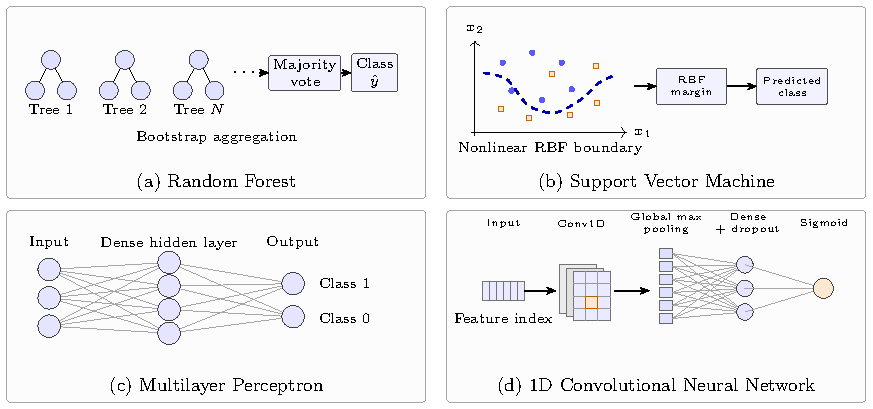
\includegraphics[width=0.9\linewidth]{figures/classifier_backbones_vector.pdf}
    \caption{Architectural topologies and structural decision mechanisms of the four candidate classifier
backbones evaluated under the equal-budget metaheuristic optimization framework.}
    \label{fig:classifier_backbones}
\end{figure}


\subsection{Optimizer Configuration, Search Operators, and Validation Objectives}
\label{sec:optimizerconfiguration}

To support a controlled comparison, five search paradigms were evaluated: Random Search (RS), Genetic Algorithm (GA), Particle Swarm Optimization (PSO), Differential Evolution (DE), and Grey Wolf Optimizer (GWO). All optimizers operate under a strict candidate evaluation cap of $N_{\mathrm{eval}} = 1{,}000$ per model and random seed. For all population-based algorithms (GA, PSO, DE, GWO), the population size is fixed to $N_{\mathrm{pop}} = 10$ candidates evaluated across $G = 100$ generations or iterations ($10 \times 100 = 1{,}000$ function evaluations). RS generates $N_{\mathrm{eval}} = 1{,}000$ independent uniform random samples across the search space.

Candidate vectors use the bounds stated above. Integer parameters and categorical-option indices are rounded and clipped to their admissible bounds:
\begin{equation}\label{eq:decoding_discrete}
\theta_d = \mathrm{clip}\!\left(\mathrm{round}(u_d),\theta_{d,\mathrm{min}},\theta_{d,\mathrm{max}}\right).
\end{equation}
For continuous parameters defined on logarithmic scales (such as $C$, $\alpha$, and learning rates), optimizers act on $u_d\in[\log_{10}(\theta_{d,\mathrm{min}}),\log_{10}(\theta_{d,\mathrm{max}})]$ and values are decoded by
\begin{equation}\label{eq:decoding_log}
\theta_d = 10^{u_d}.
\end{equation}

The specific search operators and update formulations governing each optimizer are defined as follows:
\begin{itemize}
    \item \textbf{Genetic Algorithm (GA)}: Utilizes tournament selection ($k=3$), uniform crossover with probability $P_c = 0.80$, and mutation with probability $P_m = 0.20$. When a gene is mutated, its perturbation scale is 0.10 of the corresponding encoded search range.
    \item \textbf{Particle Swarm Optimization (PSO)}: Velocity vectors $\mathbf{v}_i$ and positions $\mathbf{u}_i$ for particle $i$ at iteration $g$ are updated using inertia weight $w = 0.70$ and cognitive/social coefficients $c_1 = c_2 = 1.50$:
    \begin{equation}\label{eq:pso_update}
    \mathbf{v}_i^{g+1} = w \mathbf{v}_i^g + c_1 r_1 (\mathbf{pbest}_i - \mathbf{u}_i^g) + c_2 r_2 (\mathbf{gbest} - \mathbf{u}_i^g),
    \end{equation}
    \begin{equation}
    \mathbf{u}_i^{g+1} = \mathrm{clip}\left(\mathbf{u}_i^g + \mathbf{v}_i^{g+1}, 0, 1\right),
    \end{equation}
    where $r_1, r_2 \sim U(0, 1)$.
    \item \textbf{Differential Evolution (DE)}: Implements the DE/best/1/bin strategy with mutation factor $F = 0.80$ and binomial crossover probability $CR = 0.90$:
    \begin{equation}\label{eq:de_update}
    \mathbf{v}_i^{g+1} = \mathbf{gbest}^g + F (\mathbf{u}_{r1}^g - \mathbf{u}_{r2}^g),
    \end{equation}
    where $r1, r2$ are distinct randomly chosen population indices.
    \item \textbf{Grey Wolf Optimizer (GWO)}: Candidate position vectors are updated by simulating encirclement of the three leading wolves ($\bm{\alpha}, \bm{\beta}, \bm{\delta}$):
    \begin{equation}\label{eq:gwo_update}
    \mathbf{u}_i^{g+1} = \frac{\mathbf{x}_1 + \mathbf{x}_2 + \mathbf{x}_3}{3},
    \end{equation}
    where $\mathbf{x}_1 = \bm{\alpha} - \mathbf{A}_1 \cdot |\mathbf{C}_1 \cdot \bm{\alpha} - \mathbf{u}_i^g|$, with analogous terms for $\mathbf{x}_2$ ($\bm{\beta}$) and $\mathbf{x}_3$ ($\bm{\delta}$).
\end{itemize}

Candidate configurations are evaluated against two separated validation objectives:
\begin{itemize}
    \item \textbf{Protocol A (MCC/$F_1$ Fitness)}:
    \begin{equation}\label{eq:fitness_protocol_a}
    f_{\mathrm{MCC/F1}}(\boldsymbol{\theta}) = 0.60\,\mathrm{MCC}_{\mathrm{val}}(\boldsymbol{\theta}) + 0.40\,F_{1,\mathrm{val}}(\boldsymbol{\theta}).
    \end{equation}
    \item \textbf{Protocol B (Weighted-Accuracy Fitness)}:
    \begin{equation}\label{eq:fitness_protocol_b}
    f_{\mathrm{Acc}}(\boldsymbol{\theta}) = 0.40\,\mathrm{Accuracy}_{\mathrm{train}}(\boldsymbol{\theta}) + 0.60\,\mathrm{Accuracy}_{\mathrm{val}}(\boldsymbol{\theta}).
    \end{equation}
\end{itemize}

In addition to the two primary holdout protocols, Experiment 3 uses a separate exploratory weighted-accuracy objective with three-fold expanding-window temporal cross-validation on the concatenated training and validation observations ($N=12{,}045$). For each fold, the candidate is fitted to the earlier portion and scored on the subsequent portion; its objective is the mean of $0.40\,\mathrm{Accuracy}_{\mathrm{train}}+0.60\,\mathrm{Accuracy}_{\mathrm{validation}}$ across folds. The test feature rows are excluded from candidate selection and the selected candidate is refitted on all training-plus-validation observations before test scoring. The folds were not purged for the one-row target shift: in each fold, the last training row's target is taken from the first validation row. Experiment 3 is reported separately because its selection protocol differs from the two holdout protocols.

The two primary holdout protocols differ in both the metric and the data contribution to fitness: Protocol A uses validation MCC/$F_1$, whereas Protocol B combines in-sample training accuracy and validation accuracy. Their outcome contrast therefore describes two complete selection protocols and does not isolate the effect of changing the metric alone.

Upon completion of the $N_{\mathrm{eval}} = 1{,}000$ search budget, the optimal candidate vector $\boldsymbol{\theta}^* = \arg\max f(\boldsymbol{\theta})$ is refit on the concatenated training and validation dataset ($N = 12{,}045$ bars) and evaluated on the nominal test block ($N = 3{,}012$ feature bars). For the exploratory economic assessment, the prediction generated after bar $t$ closes is applied to bar $t+1$: an uptrend prediction opens a long position at the next bar's open, while a downtrend prediction opens a short position; each position is closed at that bar's close. The next-bar replay therefore contains at most 3,011 trades from the 3,012-row test block. Each round trip is charged a fixed cost of five index points. We report total net profit, maximum drawdown, profit factor, and annualized daily point-P\&L Sharpe ratio, computed as $\sqrt{252}\,\bar{R}_{d}/s_{d}$ from daily net point totals. These values describe this simplified one-bar execution rule, not deployable live performance. The target uses pivot-defined regime labels, whose endpoint is confirmed retrospectively; the temporal boundary implications of that labeling procedure remain a limitation of this benchmark.

\subsubsection{Asymptotic search overhead}
Let $d_s$ denote the number of encoded hyperparameters in a search space, $P$ the population size, and $G$ the number of generations or iterations. For RS, GA, PSO, and GWO, sampling and updating candidate vectors requires $O(N_{\mathrm{eval}}d_s)$ arithmetic operations when population size and tournament size are fixed; bookkeeping over fitness values adds at most $O(N_{\mathrm{eval}})$. DE also performs $O(N_{\mathrm{eval}}d_s)$ mutation, crossover, and selection work. The present DE implementation additionally constructs a list of eligible peers for each target vector, giving an implementation-specific $O(GP^2)$ bookkeeping term. Since $P=10$ is fixed in this benchmark and $N_{\mathrm{eval}}=PG$, this term is linear in the number of evaluations here. Thus, the optimizer-side overhead of all five methods is linear in $N_{\mathrm{eval}}$ for the fixed benchmark settings; this statement does not imply equal wall-clock cost.

The dominant computational cost is candidate-model fitting, not optimizer-vector arithmetic. A useful cost decomposition is $C_{\mathrm{total}}=N_{\mathrm{fit}}\,C_{\mathrm{fit}}(m,n,\boldsymbol{\theta})+C_{\mathrm{search}}$, where $m$ is the backbone, $n$ is the number of fitting observations, $\boldsymbol{\theta}$ is the candidate configuration, and $N_{\mathrm{fit}}$ counts uncached fits (three fits per uncached candidate in Experiment 3). Because RF, SVM, MLP, and 1D-CNN have different data- and parameter-dependent training costs, one common closed-form training complexity would be misleading. We therefore report an empirical fit-count measure alongside the asymptotic optimizer overhead. The candidate logs also record fit-level training seconds, used in the complementary normalized overview, but they do not provide controlled end-to-end wall-clock comparisons that include optimizer bookkeeping and orchestration.
\subsubsection{Empirical search effort}
\label{sec:empirical_effort}
The equal $N_{\mathrm{eval}}$ budget counts objective calls, but repeated candidate configurations may be served from the evaluation cache. We therefore distinguish objective calls from actual candidate-model fits. For each model--optimizer--seed run, we record the first candidate at which best-so-far validation fitness reaches 95\% of that run's total observed improvement. If $b_1$ and $b_T$ denote the initial and final best-so-far fitness, the threshold is $b_1+0.95(b_T-b_1)$. Calls to threshold equal the candidate evaluation index; actual fits equal cumulative cache misses through that index, multiplied by three for Experiment 3 (one fit per temporal fold) and one for each holdout experiment. The final refit for test evaluation is excluded. Thus, 95\% is a run-relative validation-fitness convergence threshold: it is not a 95\% test accuracy or a target defined from test performance. Held-out test metrics are computed separately after configuration selection. Values are summarized by the median across the three seeds and interpreted descriptively.

\subsection{Statistical Analysis}
\label{sec:statistical_analysis}

Statistical comparisons are conducted separately within each holdout protocol and use the four classifier backbones as the groups of interest. For a given endpoint, each optimizer--seed pair defines one matched block, giving 15 blocks (five optimizers and three seeds) per protocol. We first apply the Friedman rank test to assess whether model outcomes differ across these matched blocks. When summarizing pairwise contrasts, the model with the highest marginal mean for the endpoint is compared with each of the other three models using two-sided paired Wilcoxon signed-rank tests. The resulting three $p$-values are adjusted together using the Holm step-down procedure, with family-wise significance level $\alpha=0.05$.

These tests are exploratory. The blocks share one chronological test segment, and the five optimizers and three seeds do not provide 15 independent market periods. Accordingly, the tests quantify consistency of model ordering across the evaluated optimizer--seed combinations on this fixed test period; they do not establish replication across market regimes or a confirmatory difference between validation protocols. No optimizer-superiority claim is inferred from these model-level tests.
